\section{Methodology}

\section{Implementation}


\subsection{Code Schematic}

\begin{figure}[h]
\centering
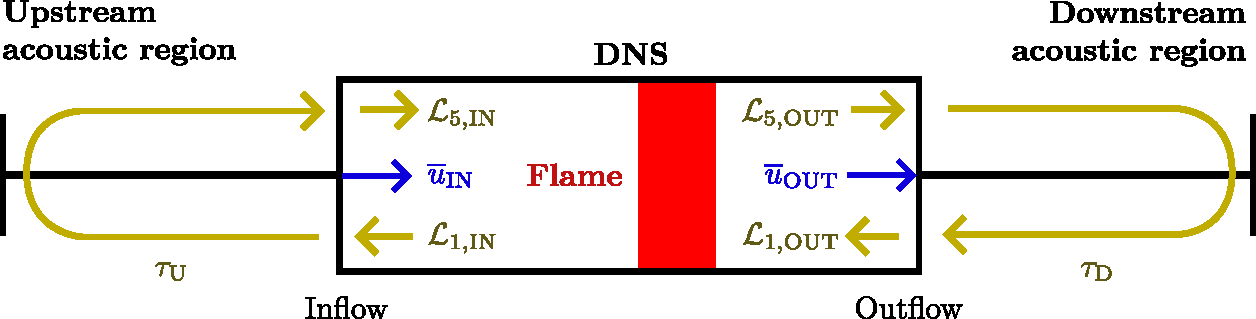
\includegraphics[scale=0.6]{assets/imgs/delay_bc_model.pdf}
\label{fig:delay-model}
\caption{}
\end{figure}

\begin{figure}[h]
\centering
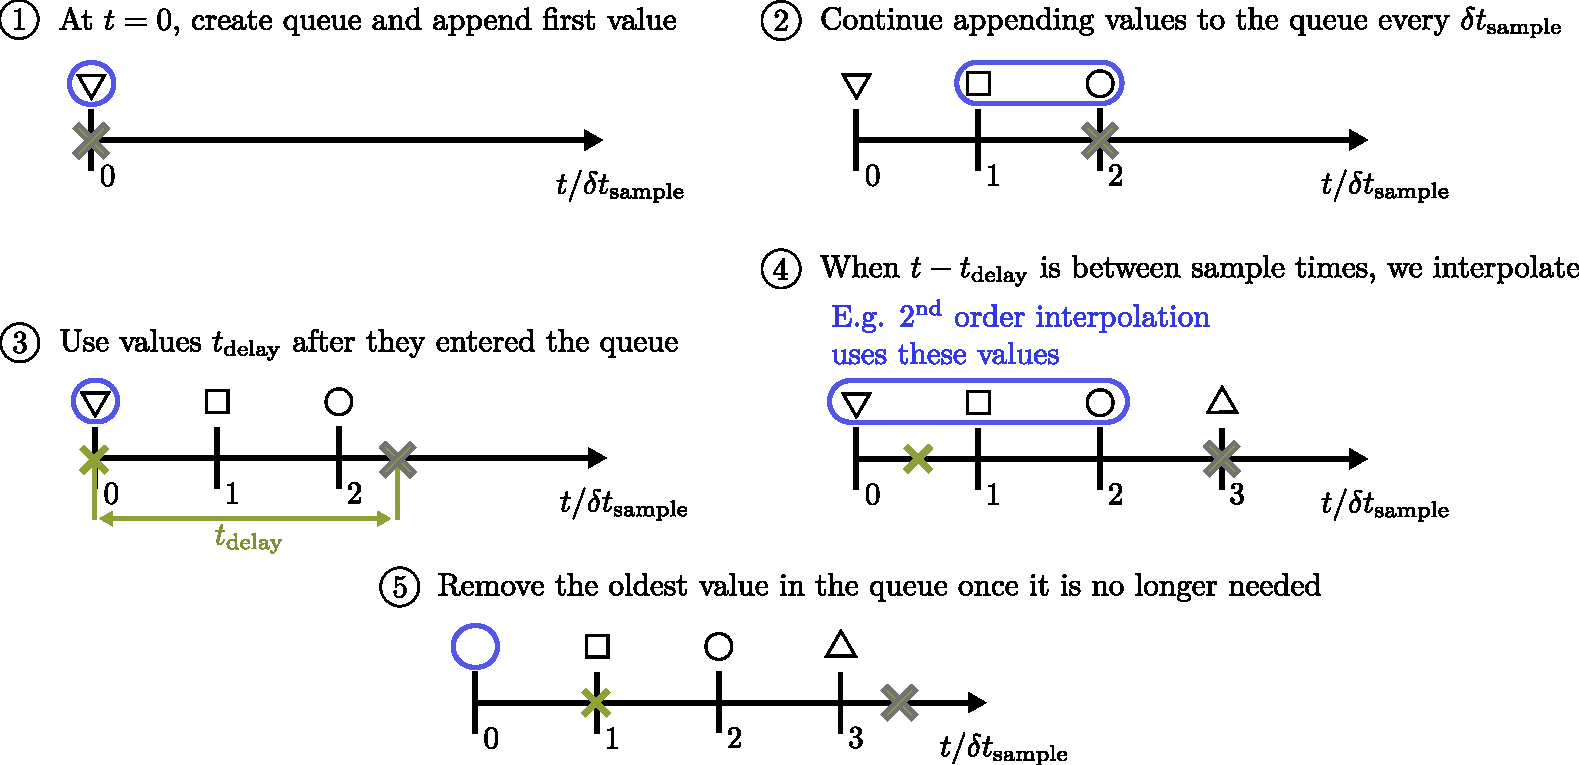
\includegraphics[scale=0.6]{assets/imgs/delay_bc_queue.pdf}
\label{fig:delay-queue}
\caption{}
\end{figure}

\begin{figure}[h]
\centering
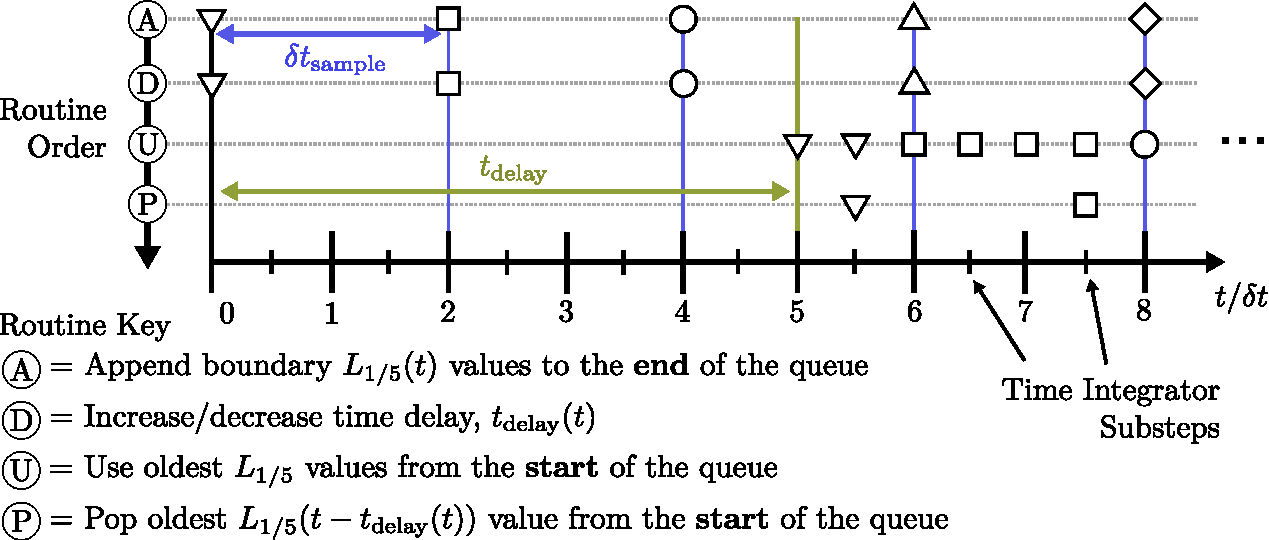
\includegraphics[scale=0.6]{assets/imgs/delay_bc_code_schematic.pdf}
\label{fig:schematic}
\caption{Schematic for delay BCs implemented into a multistage time integrator. }
\end{figure}


\begin{itemize}
\item Queues are filled with $L$ values as well as 
\end{itemize}



\subsection{Overcoming Instabilities}



\subsection{Sampling Error}




